\chapter{Proponowany system wizyjny}
\label{cha:propSysWiz}


\begin{figure}
\centering
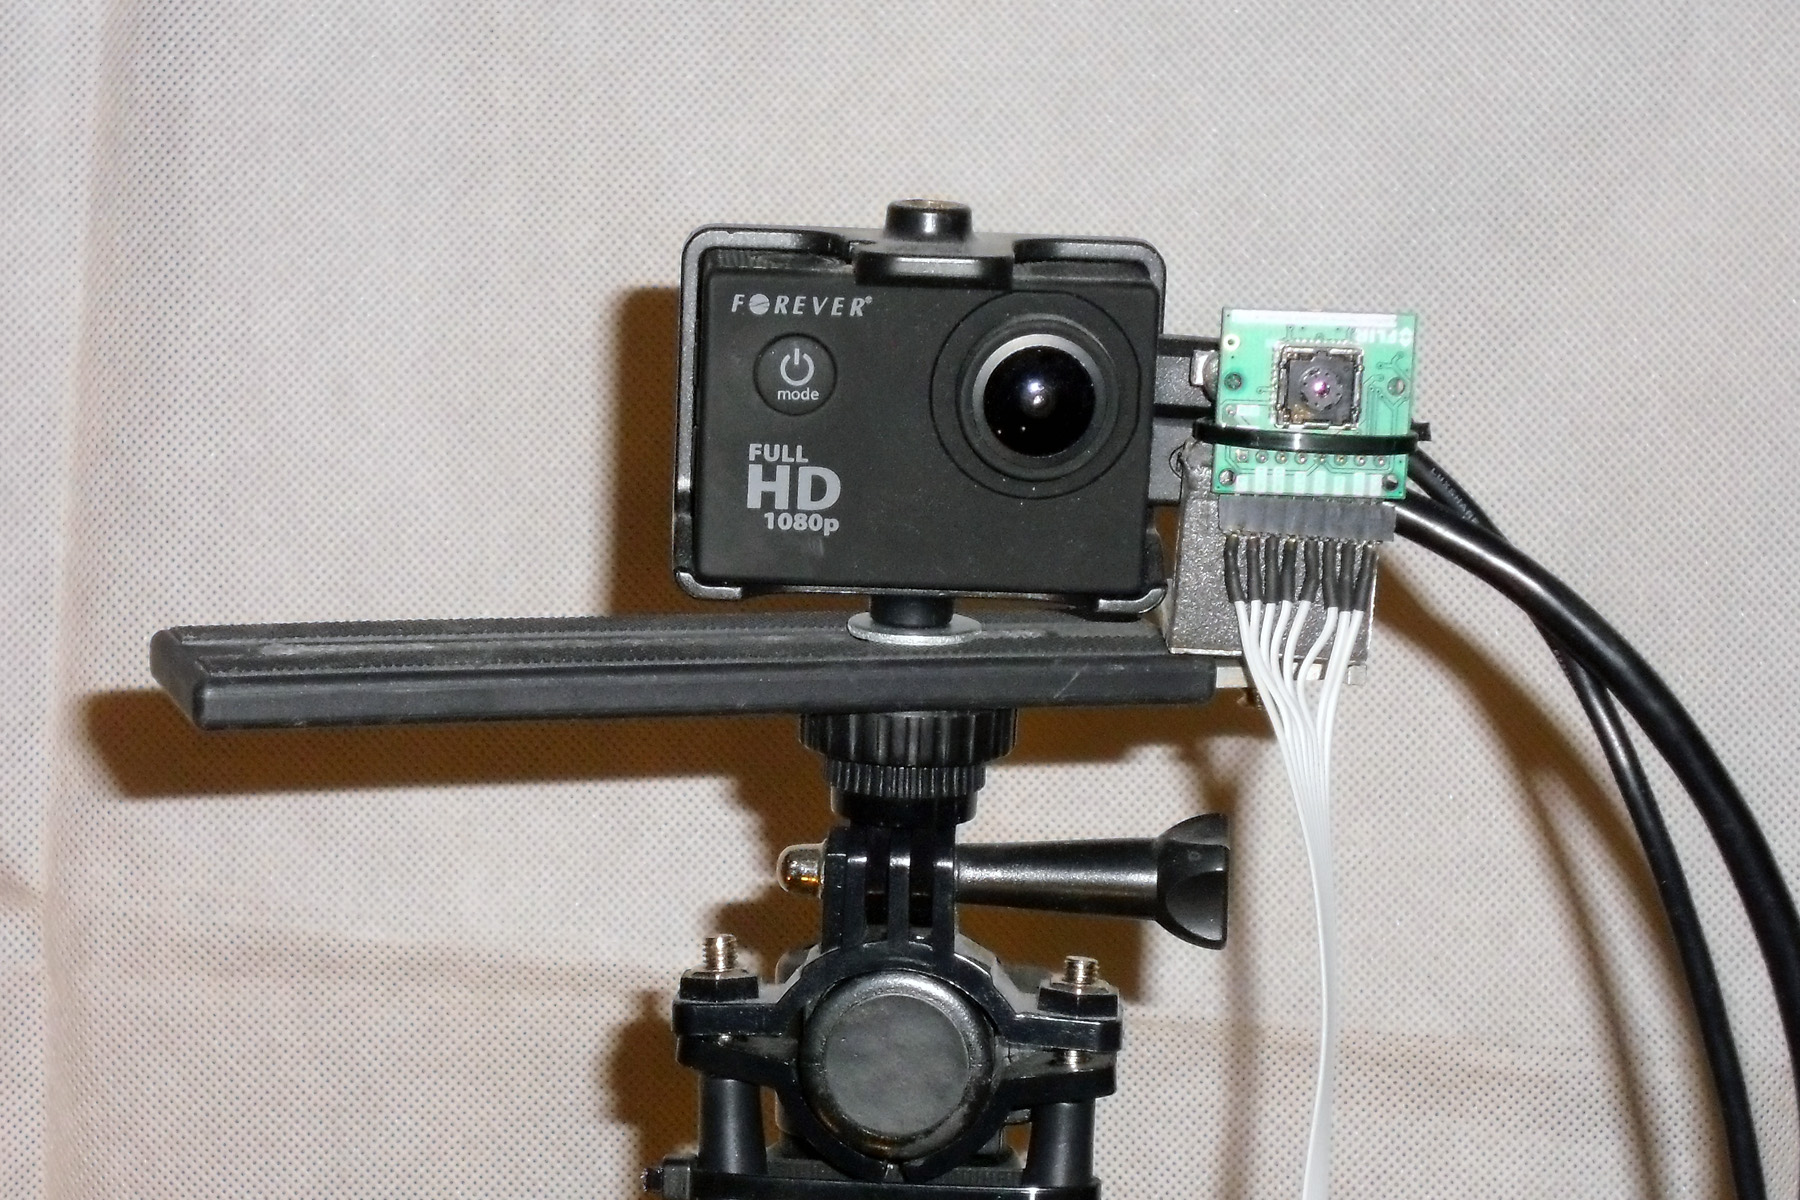
\includegraphics[width=0.65\linewidth]{images/kameraRGBIR.jpg}
\caption[Wykożystany system kamer.]{Wykożystany system kamer. Po lewej stronie znajduje się kamera wizyjna, po prawej termowizyjna Lepton.}
\label{fig:kameraRGBIR}
\end{figure}

\begin{figure}
\centering
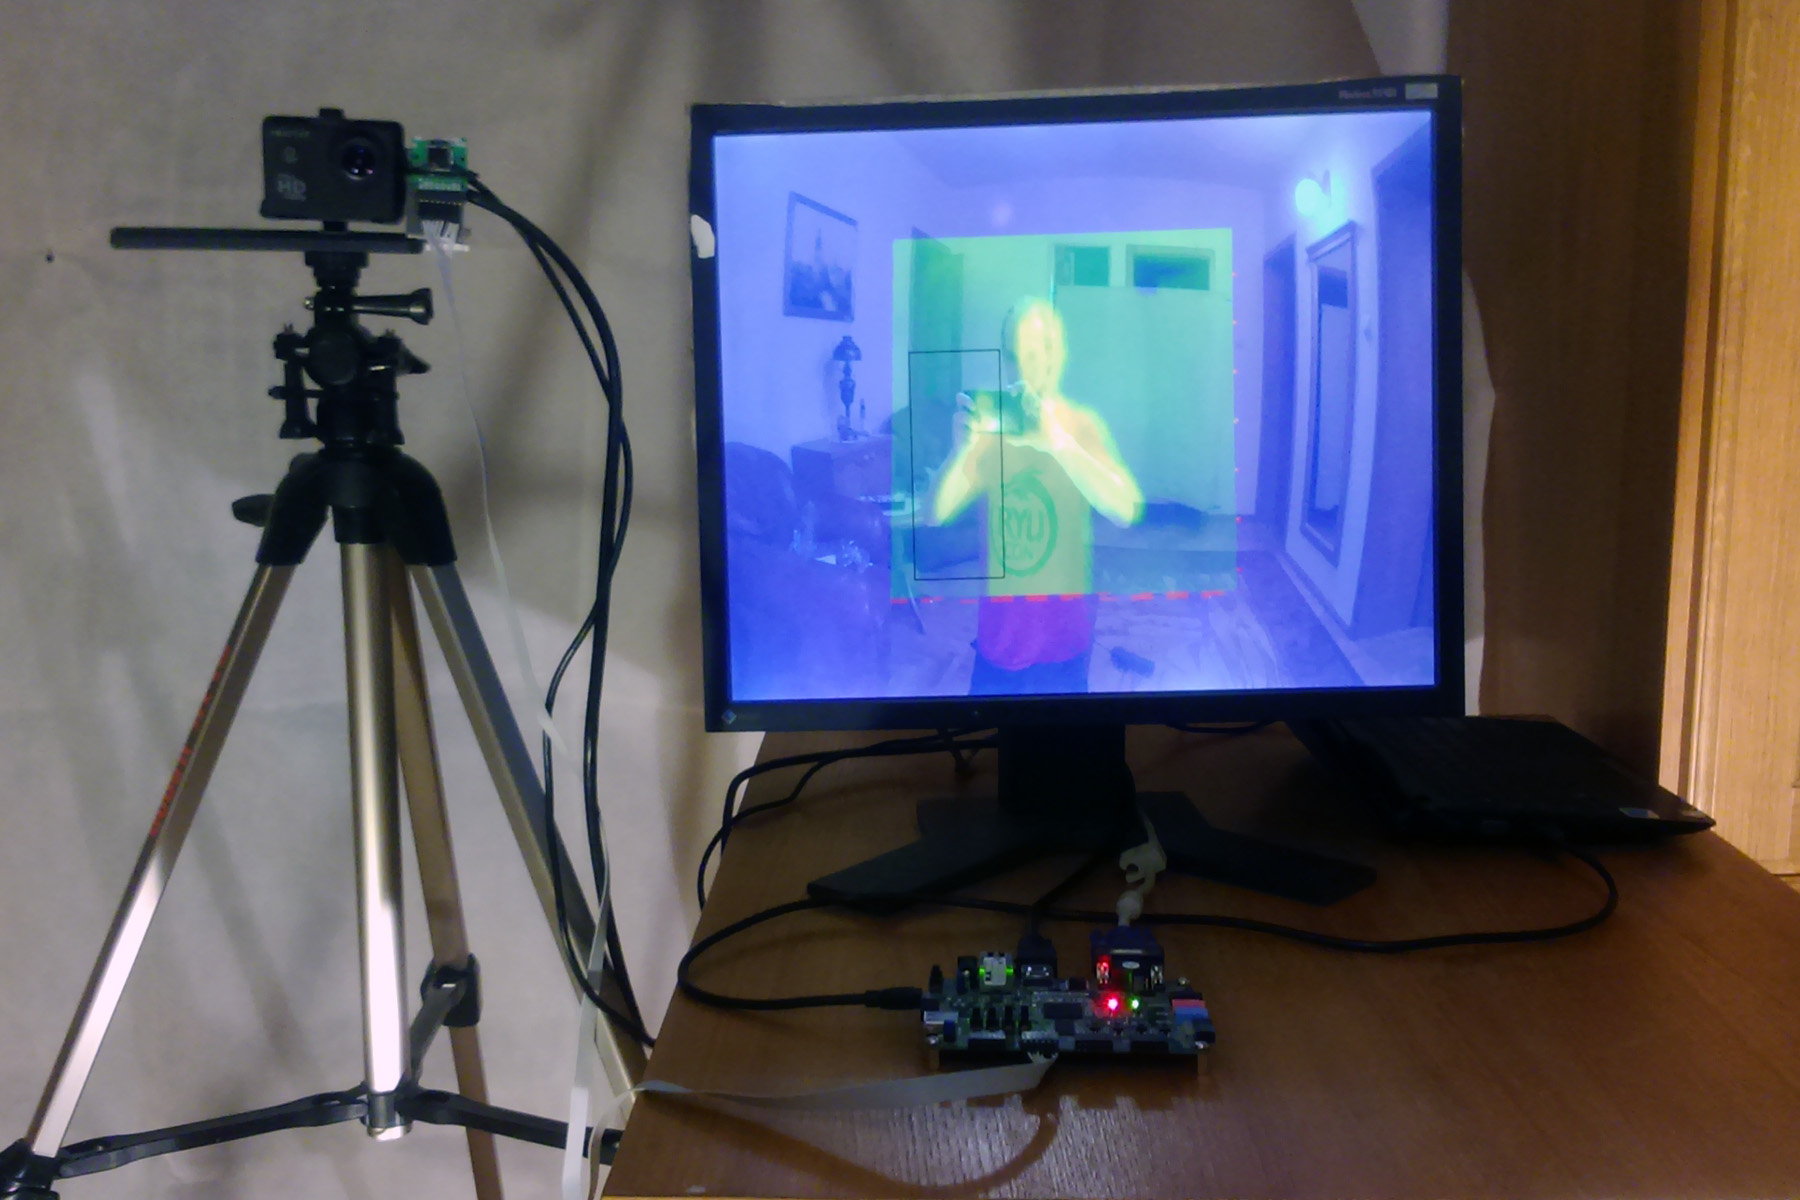
\includegraphics[width=0.65\linewidth]{images/systemOverview.jpg}
\caption[Widok na kompletny system.]{Widok na kompletny system do detekcji obiektów w przestrzeni multispektralnej. Obraz jest rejestrowany przez zespół kamer znajdujący się na statywie. Kamery są połączone do płytki deweloperskiej Zybo. Wynik jest prezentowany na monitorze.}
\label{fig:systemOverview}
\end{figure}



\section{Koncepcja systemu}
Zadaniem systemu jest detekcja osób w obrazie multispektralnym. Do uzyskania obrazu multisprktralnego została wykorzystana kamera wizyjna, dająca obraz parametrach 640x480px i 50 klatek na sekundę oraz termowizyjna: Lepton – 80x60px i 9 klatek na sekundę. Obraz z kamery termowizyjnej (IR) jest dopasowywany do wizyjnego (RGB) za pomocą projekcji perspektywicznej. Wynikiem ich połączenia jest obraz multispektralny (RGBIR). Wybór ROI odbywa się tylko z wykorzystaniem obrazu termowizyjnego. W tym celu został wykorzystany moduł PDM (ang \textit{Probability Density Matrix}) zaczerpnięty z pracy inżynierskiej autora \cite{kankaing}.Tworzy on listę kandydatów z której jest wybierany najbardziej prawdopodobny wynik. Następnie z ROI o wymiarach 80x192px są wyodrębniane deskryptory HOG oraz odbywa się klasyfikacja z wykorzystaniem SVM. Wynik detekcji jest prezentowany na ekranie, poprzez obramowanie sylwetki przechodnia.
Do realizacji tego systemu została wykorzystana płytka deweloperska ZYBO firmy Digilent. Bazuje ona na omówionym wcześniej w rozdziale \ref{cha:fpga} układzie Zynq-7000. Jest to układ heterogeniczny co daje możliwość realizacji poszczególnych elementów systemu wizyjnego w logice programowalnej (PL) lub systemie procesorowym (PS) 
Zaproponowano następujący podział zadań:

Logika programowalna :
\begin{itemize}
\item Akwizycja obrazu poprzez HDMI (RGB) i VoSPI (IR),
\item Transformata projekcyjna i interpolacja obrazu IR,
\item Nałożenie i synchronizacja obrazu IR do obrazu RGB,
\item Prezentacja wyników,
\item Detekcja kandydatów za pomocą wzorca probabilistycznego.
\end{itemize}
System procesorowy:
\begin{itemize}
\item konfiguracja parametrów systemu wizyjnego w logice programowalnej poprzez interfejs AXI4-Lite,
\item Klasyfikacja obszarów wytypowanych przez wzorzec probabilistyczny,
\item Generowanie wyników.
\end{itemize}
\begin{figure}[h]
    \centering
    \includegraphics[width=1\textwidth]{images/system}
    \caption{Schemat blokowy systemu detekcji.}
    \label{fig:systemwizyjny}
\end{figure}

Na rysunku \ref{fig:systemwizyjny} został przestawiony ogólny schemat rozwiązania.
%TODO OK To bym przerzucił to rozdziału, gdzie Pan opisuje system. 
\section{Wykorzystanie AXI-Stream do transmisji sygnału wideo.} 
W odróżnieniu od standardowego sposobu przetwarzania strumieniowego wideo, w AXI4-Stream przesyłane są jedynie aktywne piksele. 
%TODO raczej od standardowego sdposobu przesyłania danych wizyjnych.
Linie synchronizacji poziomej i pionowej są odrzucane albo przekierowywane do specjalnego bloku w którym są mierzone parametry wchodzącego strumienia wizyjnego (liczba pikseli w~linii, liczba aktywnych linii, czas wyciemnienia itd.). 
W celu wyświetlenia obrazu, wykorzystuje się ten sam blok w celu generacji nowych sygnałów synchronizacji. 
%TODO OK timining - do wymiany. Musi Pan to lepiej przedstawieć, tzn. że takie przychodzi z kamery, można to usunąć, ale trzeba odtworzyć aby wyświetlić.

Do transmisji wykorzystane jest 6 sygnałów: dane i pięć kontrolno-sterujących. W nawiasach są podane linie które wykorzystuje dany sygnał w interfejsie AXI4-Stream.
\begin{itemize}
\item \textit{Video Data} (\textit{tdata})-- linia danych o szerokości jednego (albo dwóch) pikseli. Szerokość tej linii powinna być wielokrotnością liczby osiem (16, 24, 48 itd.)
\item \textit{Valid}(\textit{tvalid}) -- linia określająca czy dane piksela są poprawne,
\item \textit{Ready} (\textit{tready})-- linia kontrolna informująca urządzenie master, że \textit{slave} jest gotowy do transmisji danych, %TODO kursywa
\item \textit{Start Of Frame} (\textit{tuser}) -- linia, która wskazuje pierwszy piksel nowej ramki,
\item \textit{End Of Line} (\textit{tlast})-- linia wskazująca ostatni piksel w linii. %TODO tu i wyżej "wskazuje" to złe słowo.

\end{itemize}
%TODO Ogólnie nazwy tych linii (wszystkich) kursywą
Aby mógł wystąpić poprawny transfer danych linie \textit{Valid} i \textit{Ready} muszą być w stanie wysokim podczas rosnącego zbocza zegara. 
Przykładowe nawiązanie transmisji przedstawia rysunek \ref{fig:handshake}

\begin{figure}[h]
    \centering
    \includegraphics[width=1\textwidth]{images/axi-stream_hendshake}
    \caption{Przykład rozpoczęcia transmisji Reday/Valid.}
    \label{fig:handshake}
\end{figure}

%TODO To też to tej cześci implementacyjnej
\section{AXI VDMA}
Wiele aplikacji wizyjnych wymaga przechowania całej ramki obrazu w celu jej dalszej obróbki np. podczas skalowania, przycinania bądź dopasowania liczby klatek na sekundę. 
Część programowalna układu Zynq zazwyczaj nie posiada wystarczającej liczby zasobów pamięciowych do przechowanie pełnej klatki obrazu w swojej strukturze. 
Aby stworzyć taki bufor jest wykorzystywany mechanizm bezpośredniego dostępu do pamięci, który pozwala na przesłanie i wczytanie danych z logiki programowalnej do pamięci RAM bez konieczności angażowania procesora. 
%TODO OK tym - tzn. jakim (niejasne)
Realizuje się to poprzez IP-Core AXI VDMA. 
Zapewnia on przejście między interfejsem AXI4-Stream, a AXI4 Memory Map w obu kierunkach. 
Przed rozpoczęciem przesyłania IP-Core jest konfigurowany poprzez interfejs AXI4-Lite. 
Konfiguracja zawiera adres w pamięci RAM do którego ma być zapisana bądź wczytana ramka obrazu. 
Po wgraniu do pamięci ramki kontroler może wywołać przerwanie dla systemu procesorowego.
\section{Opis modułów w logice programowalnej}
\subsection{Kontroler kamery IR}
Kamera Lepton przesyła obraz za pomocą interfejsu VoSPI (ang. \textit{Video over Serial Peripheral Interface}). Kamera jest urządzeniem typu \textit{slave}, zaś układ ZYNQ jest \textit{master}. Są wykorzystywane 3 z 4 linii typowego kanału SPI: SCK (ang. \textit{Serial Cloack} – zegar), /CS (ang. \textit{Chip Select} -- wybór układu)(aktywny stanem nikim) oraz MISO (ang. {Master In/Slave Out} – wejście master/wyjście slave).
Transmisja rozpoczyna się od podania stanu niskiego przez kontroler na linii /CS. Powoduje to aktywację linii. Następnie, \textit{master} rozpoczyna taktowanie zegarem na linii SCK. \textit{Slave} wystawia kolejne bity danych począwszy od MSB (ang. \textit{most significant bit}) na linię MISO. Kontroler szczytuje te bity przy każdym rosnącym zboczu zegara do 16 bitowego rejestru przesuwnego.
Dane przesyłane z kamery są zorganizowane w pakiety po 164 bajty. Rozpoczęty jest nagłówkiem składającym się z 2 bajtów pola identyfikacyjnego oraz 2 bajtami sumy CRC. Pole identyfikacyjne spełnia dwa zadania. Po pierwsze, stanowi 12 bitowy numer pakietu (a zarazem numer linii obrazu), po drugie, w przypadku błędnego pakietu zawiera wartość 0xXFXX (X to obojętna wartość) co wskazuje że nadchodzący pakiet powinien zostać zignorowany przez kontroler. Zawartość pakietu stanowi 160 bajtów zawierających wartości 80 pikseli linii. W systemie wykorzystywany jest format RAW14, więc każdy piksel jest przesyłany w postaci 2 bajtów zawierających 14 bitową wartość piksela. 
Cała ramka obrazu składa się z 63 pakietów. 60 pierwszych pakietów stanowią linie obrazu zaś ostatnie 3 są przeznaczone na telemetrię, która zawiera m.in. temperaturę FPA i obudowy, 32-bitowy licznik ramek obrazu i bity stanu. 
Pierwsze 3 przesłane pakiety są błędne i służą do synchronizacji transmisji. 
W przypadku prawidłowego pakietu kontroler szczytuję numer linii obrazu i wystawia go na wyjściu \textit{row}. Następnie na wyjściu \textit{data} wystawiane są wartości kolejnych 80 bitów wraz z ich pozycją na wyjściu \textit{column}. Wysoki stan \textit{we} informuje że dane są poprawne i powinny być zapisane. 
\textit{Row} i \textit{column} są zamieniane na adres w pamięci dwuportowej, będącą buforem ramki IR, do której są zapisywana wartość piksela z wyjścia \textit{data}.

\subsection {Transformata projekcyjna}
Moduł ma na celu dopasowanie obrazu IR do RGB. W tym celu zamienia współrzędne w układzie odniesienia obrazu RGB na odpowiadające im w układzie IR.
%TODO OK styl.
Na wejściu podawany jest strumień AXI4-Stream służący do synchronizacji ramek oraz 12 bitowe współrzędne X i Y. %TODO OK timinig (zmienić słowo)
Moduł realizuję operację: 
\begin{equation}
\begin{bmatrix}
u_n & v_n & n
\end{bmatrix} 
= 
\begin{bmatrix}
x & y & 1
\end{bmatrix}
T
\end{equation}

\begin{equation}
u = \frac{u_n}{n}
\end{equation}

\begin{equation}
v = \frac{v_n}{n}
\end{equation}

\noindent
 gdzie $x$,$y$ to współrzędne obrazu w układzie odniesienia kamery wizyjnej, $u$,$v$ to odpowiadające im współrzędne w układzie odniesienie kamery termowizyjnej. $T$ to macierz transformacji.
%TODO OKopisać te symbiole

Moduł wystawia na wyjściu strumień wizyjny AXI4-Stream, 12 bitowe wartości U i V oraz ich części ułamkowe w U\_fraction i V\_fraction (14 bitów). %TODO OK tez to timinigów.
W module zostały wykorzystane 34 z 80 dostępnych w układzie Zynq modułów DSP48 do wykonania operacji arytmetycznych, z czego większość została zutylizowana przez IP-Core dzielarki dostarczony od producenta układu. %TODO OK modułów DSP48 
%% Do implementacji jednej dzielarki zostało wykorzystane 14 modułów DSP. %TODO OK powt. to jakoś trzeba złączyć z poprzednim 
Dzielenie nie odbywa się w pełni potokowo. Użyty w dzielarce algorytm High\_Radix wymaga zatrzymania strumienia na czas obliczeń. Zmniejszenie ilości instancji dzielarek pozwoliło na zaoszczędzenie pewnej ilości (jak się później okazało istotnej) zasobów logicznych.
Jednak dzięki zastosowaniu wyższej częstotliwości niż zegar pikseli obrazu RGB oraz bufora (250 MHz) nie stanowi to wąskiego gardła systemu. %TODO a w innym trybie to nie działa w pełni potokow ? Swoją drogą, czy nie można jakoś tego uniknąć ? %% TT Początkowo działo w pełni potokowo ale musiałem to zmienić bo mi brakło zasobów(może nie brakło ale nie dało się zsyntezować)
Macierz transformacji T jest zapisana w dziewięciu 32 bitowych rejestrach i konfigurowalna poprzez interfejs AXI4-Lite. 
Elementy macierzy są 25 liczbami w notacji stałoprzecinkowej: 1 bit znaku 10 – część całkowita, 14 – część ułamkowa. Taka dokładność pozwala na maksymalne wykorzystanie pojedynczych modułów DSP48 (gdyż wejćie B jest 25-bitowe). Rysunek \ref{fig:transfProjek} przedstawia schemat modułu.
\begin{figure}
\centering
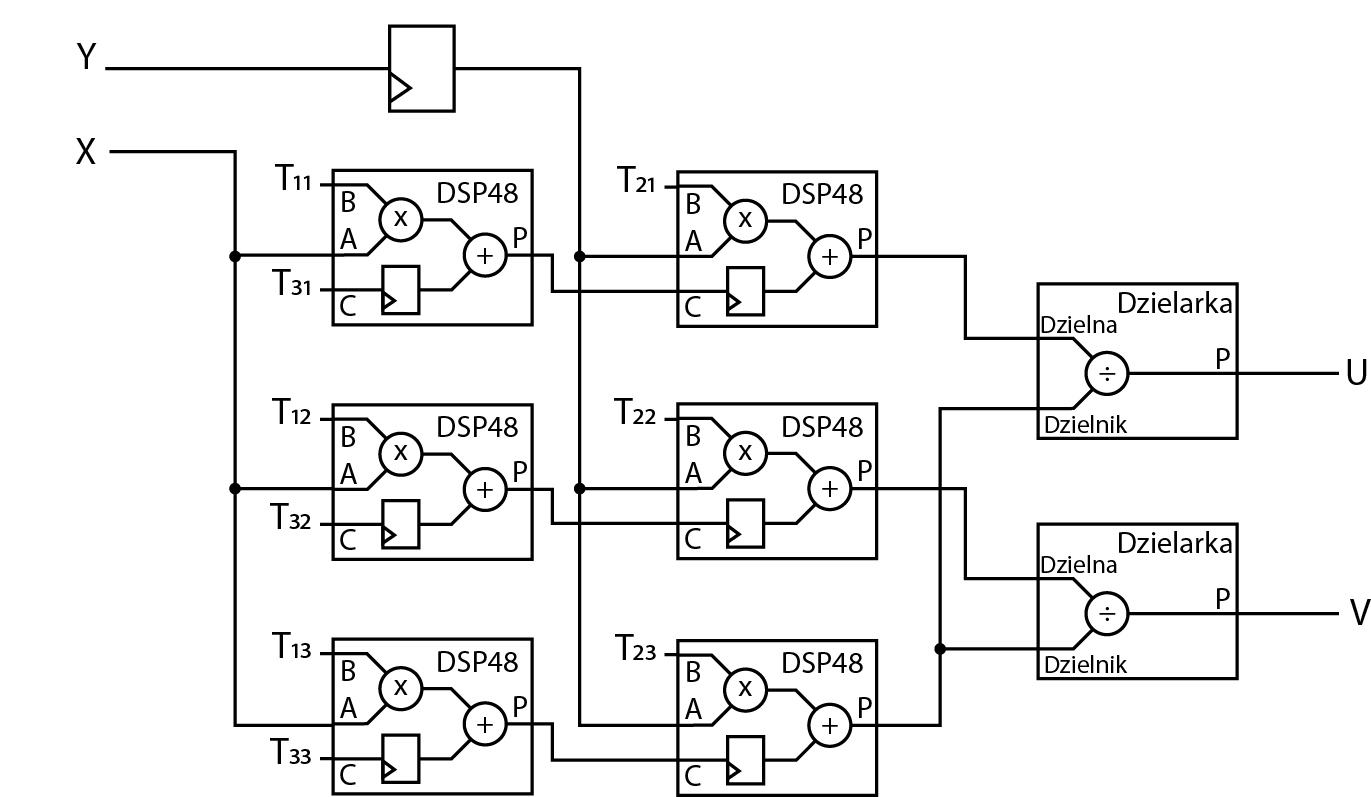
\includegraphics[width=0.70\linewidth]{images/transfProjek.png}
\caption[Schemat modułu transformacji projekcyjnej.]{Schemat modułu transformacji projekcyjnej.}
\label{fig:transfProjek}
\end{figure}
%TODO OK Też jakiś schemat obliczeń i więcej szczegółów.
\subsection{Interpolacja dwuliniowa} %TODO OK może lepiej dwuliniowa
%% Ma za zadanie pobrać z pamięci dwuportowej obrazu IR wartość piksela wskazaną na wejściu układu i wystawić na wyjście. %TODO OK??? a coś jeszzce zrobić - bo to jest kontorler....
Pozwala na interpolacje wartości piksela wskazanego przez koordynaty na wejściu modułu.
Podobnie jak reszta systemu używa AXI4-Stream do przekazywania danych między poszczególnymi modułami. 
Dane na wejściu to współrzędne U i V oraz ich części ułamkowe U\_fraction ($U_f$) i V\_fraction ($V_f$). 
Moduł został wyposażony w 4 rejestry, w których przechowywane są współrzędne oraz wartości 4 ostatnio użytych pikseli. 
Zabieg ten znacznie redukuje liczbę potrzebnych zapytań do pamięci. 
Podczas powiększania obrazów jest duża szansa, że kolejne koordynaty na wejściu U, V odwołają się do tych samych czterech otaczających ich pikseli. Podczas transformacji dużego obrazu na mniejszy kolejne piksele obrazu wejściowego (np.(0,0), (1,0), (2,0), ...) odwołują się do przestrzeni pomiędzy czteroma pikselami małego obrazu (np. podczas zmniejszenia 10-krotnego wynikiem transformacji byłyby punkty: (0,0), (0.1,0), (0.2,0), ...) więc w celu interpolacji odwoływały by się do wartości pikseli (0,0) , (1,0), (0,1), (1,1)). 
%TODO OK napisac dlaczego tak jest
W module jest sprawdzane, czy w pamięci są już wartości z koordynatów [U,V], [U+1,V] [U,V+1], [U+1,V+1]. 
Jeżeli któregoś piksela brakuje, jest on pobierany z pamięci i zapisywany w rejestrze przechowującym niepotrzebny piksel. 
Jeżeli wszystkie koordynaty się zgadzają , obliczana jest wartość piksela wyjściowego zgodnie ze wzorem \eqref{equ:bilinear}.  

\begin{equation}\label{equ:bilinear}
Ir = A(1-U_{f})(1-V_{f})+B(1-V_{f})+C(1- U_{f})V_{f}+ D U_{f} V_{f}
\end{equation}
\noindent gdzie: $ A, B, C ,D $ odpowiadają wartościom pikseli w [U,V], [U+1,V] [U,V+1], [U+1,V+1], a $ Ir $ to wartość wyjściowa piksela wyjściowego, %TODO OK no to może nie wprowadzać dwóch oznaczeń (w sensie _f i _fraction, tylko ujednolicić.)

Moduł działa potokowo. W przypadku gdy jest wymagana aktualizacja rejestrów, strumień jest wstrzymywany na czas pobrania stosownych wartości z bufora ramki IR. Jeżeli koordynaty wejściowe wychodzą poza zakres obrazu termowizyjnego, to ich wartość wyjściowa odgórnie wynosi zero.
%TODO OK styl. + czegoś brakuje na początku

\subsection{Łączenie strumieni}

Moduł posiada dwa wejścia AXIS4-Steam. Strumień RGB jest nadrzędny, i do niego jest dołączany  strumień IR. %TODO OK dodać który jest który
Do synchronizacji została wykorzystana możliwość wstrzymania transmisji poprzez linię \textit{tready} w interfejsie AXI4-Stream. 
Piksele z dołączanego obrazu są odrzucane do momentu pojawienia się sygnału SOF, reprezentowanym przez wysoki stan linii \textit{tuser}. Następnie w momencie pojawienia się sygnału SOF w strumieniu głównym transmisja zostaje ponownie wznowiona. %TODO OKa) za dużo strumień, poza tym jest to jakieś niejasne.
Po przejściu całej ramki strumienie są ponownie synchronizowane.  
\subsection{Koloryzacja i nakładanie}
Strumień RGBIR zostaje połączony w jeden obraz. 
Obraz IR zostaje poddany koloryzacji na podstawie wartości zapisanych w 12-bitowym LUT(ang. \textit{Lookup table}). Rysunek \ref{fig:jetPalet} przedstawia użytą paletę do wizualizacji temperatury. Obrazy nakładają się w proporcjach 50 na 50. Jeżeli wartość piksela IR jest równa zero to nie jest wyświetlany.
Na wyjściu jest podany 24 bitowy strumień RGB. Wynik operacji jest przedstawiono na rysunku \ref{fig:koloryzacja}.
\begin{figure}
\centering
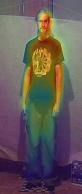
\includegraphics[width=0.3\linewidth]{images/koloryzacja.jpg}
\caption[Obraz IR po koloryzacji i nakłądaniu.]{Obraz IR po koloryzacji i nakłądaniu.}
\label{fig:koloryzacja}
\end{figure}

\begin{figure}
\centering
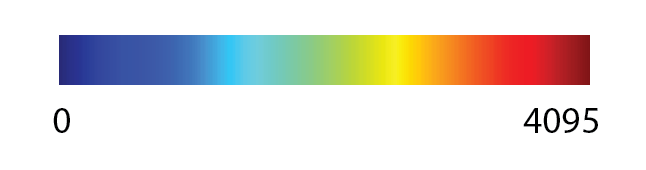
\includegraphics[width=0.5\linewidth]{images/jetPalet.png}
\caption[Paleta kolorów użyta do wizualizacji temperatury.]{ Paleta kolorów użyta do wizualizacji temperatury.}
\label{fig:jetPalet}
\end{figure}
%TODO na pewno przykład obrazu, rozwinięcie LUT, jakieś szczegółby tej koloryzacji
\subsection{Obramowanie wyników}
Moduł ma na celu wskazanie na obrazie lokalizacji wykrytego przechodnia, poprzez obramowanie tego obszaru ramką określonego koloru. Kolor, rozmiar i lokalizacja ramki jest zapisana w dwóch 32-bitowych rejestrach, konfigurowalnych poprzez interfejs AXI4-Lite. 
\subsection{Moduł DPM}
Moduł został zaczerpnięty z pracy inżynierskiej autora w celu selekcji kandydatów w obrazie multispektralnym i jest opisany w rozdziale \ref {sec:xiao_2015}.  Do detekcji wykorzystuje bezpośredni strumień pikseli kamery termowizyjnej. Pomocniczy moduł \textit{data grabber} znajdujący się tuż za kontrolerem kamery IR ma za zadanie rozdzielenie sygnału do dwóch komponentów: bufora ramki oraz, po zbinaryzowaniu, do modułu DPM wraz z jego koordynatami. Moduł składa się z okna kontekstowego o wymiarach 16x40 px, gdzie odbywa się porównanie z macierzą wzorcową. Do każdego piksela w oknie jest przypisywana jest wartość z wzorca LPBW – jeżeli piksel jest biały, albo LPMB w przypadku czarnego. Następnie wszystkie wartości są sumowane za pomocą drzewa sumacyjnego, wynikiem czego jest wartość wyjściowa LP (ang. \textit{Logarithmic Probability}). Jeżeli ta wartość przekroczy (ustaloną na podstawie sumy LP policzoną dla tła i parametru K) wartość progową zostaje przesłana do listy kandydatów wraz z współrzędnymi tego okna (w układzie odniesienia kamery IR). Lista kandydatów jest na bieżąco przesyłana za pomocą AXI4-Stream do pamięci systemu procesorowego poprzez AXI DMA. Po sprawdzeniu ostatniego okna zostaje przesłany sygnał \textit{tlast} i moduł AXI DMA wygeneruje przerwanie w systemie procesorowym. Wartość progowa binaryzacji i LP jest konfigurowalna za pomocą AXI4-Lite.
\section{System procesorowy}
Program działający w części procesorowej układu Zynq spełnia dwa podstawowe zadania. Po pierwsze pozwala na konfigurację modułów znajdujących się w PL za pomocą AXI4-Lite. Użytkownik za pośrednictwem konsoli może wprowadzać własne parametry dla każdego z modułów. Pozwala również na zapis na karcie SD pojedynczej klatki obrazu multispektralnego, następnego wykrytego ROI oraz ROI znajdującego się pośrodku sceny. Ta opcja ułatwiła tworzenie bazy do nauczenia klasyfikatora SVM. 

Drugim zadaniem jest klasyfikacja wytypowanego przez DPM kandydata. Po otrzymaniu przerwania przez moduł AXI DMA powiązany z DPM, sprawdzana jest lista kandydatów i wybierany jest ten o największej wartości LP. Współrzędne kandydata są podane w układzie odniesienia kamery IR. Po przeliczaniu ich, za pomocą macierzy transformacji projekcyjnej, i dodaniu pewnego \textit{offsetu} w buforze ramki obrazu RGBIR jest wskazany ROI o wymiarach 80x192. Następnie jest obliczany wektor cech HOG z tego obszaru. Potem na jego podstawie odbywa się klasyfikacja przy użyciu wytrenowanego SVM. Wynik klasyfikacji jest wyświetlany w konsoli wraz z jego współrzędnymi na obrazie i wartością LP. Dodatkowo obszar ten zostanie zaznaczony zieloną ramką na wyjściu monitora. Jeżeli najlepszy kandydat nie zostanie zakwalifikowany pozytywnie przez SVM ramka przybierze kolor czerwony. Brak kandydatów wskazuje czarna ramka w miejscu ostatniej detekcji. 
\section{Proces kalibracji}
W celu kalibracji, zostaje wykonane zdjęcie specjalnej planszy kalibracyjnej za pomocą obu kamer (rysunki \ref{fig:calibrationThermal}, \ref{fig:calibrationRGB}). Pozwala to na identyfikację czterech punktów kalibracyjnych w obu przestrzeniach: RGB i IR. Następnie na ich podstawie zostaje obliczona macierz transformacji projekcyjnej. Na rysunku \ref{fig:calibrationCorrectedGrey} przedstawiono obraz z kamery termowizyjnej po transformacji, który po krywa się z obrazem wizyjnym (rysunek \ref{fig:calibrationSum})

\begin{figure}[h]
	\centering
	\begin{subfigure}{0.47\textwidth}
		\centering
		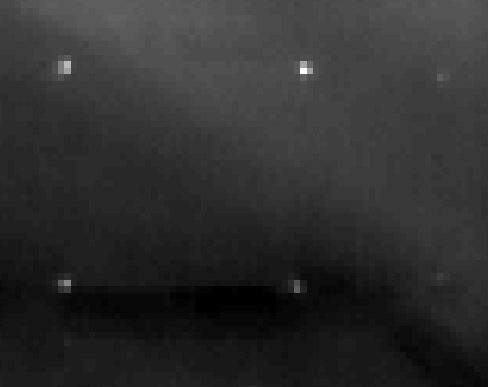
\includegraphics[width=0.9\linewidth]{images/calibrationThermal}
		\subcaption{\label{fig:calibrationThermal}}
	\end{subfigure}
	\begin{subfigure}{0.47\textwidth}
		\centering
		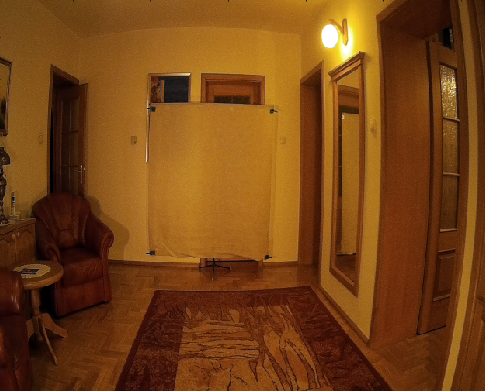
\includegraphics[width=0.9\linewidth]{images/calibrationRGB}
		\subcaption{\label{fig:calibrationRGB}}
	\end{subfigure}
	\begin{subfigure}{0.47\textwidth}
		\centering
		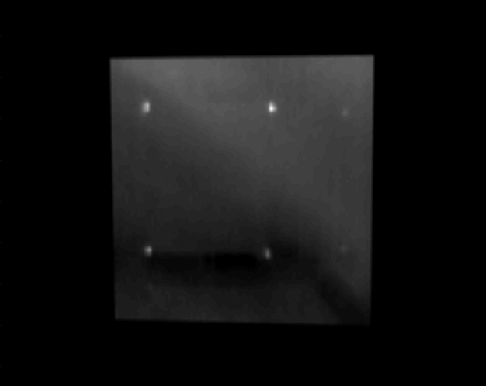
\includegraphics[width=0.9\linewidth]{images/calibrationCorrectedGrey}
		\subcaption{\label{fig:calibrationCorrectedGrey}}
	\end{subfigure}
	\begin{subfigure}{0.47\textwidth}
		\centering
		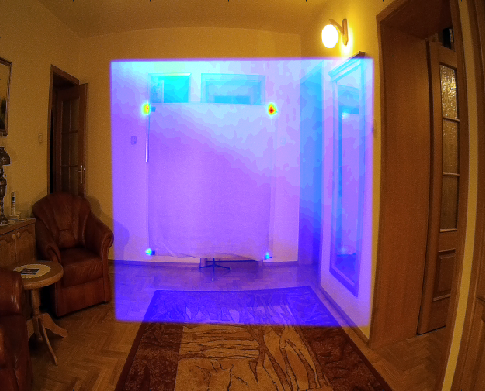
\includegraphics[width=0.9\linewidth]{images/calibrationSum}
		\subcaption{\label{fig:calibrationSum}}
	\end{subfigure}	
	\caption[Proces kalibracji]{Proces kalibracji: \protect\subref{fig:calibrationThermal} obraz z kamery termowizyjnej, \protect\subref{fig:calibrationRGB} obraz z kamery wizyjnej, \protect
\subref{fig:calibrationCorrectedGrey} obraz z kamery termowizyjnej po transformacji projekcyjnej, \protect\subref{fig:calibrationSum} obraz z kamery termowizyjnej po transformacji projekcyjnej nałożony na obraz z kamery wiyjnej.}
\end{figure}

\section{HOG i SVM}
Okno decyzyjne jest podzielone na 60 komórek o wielkości 16x16 pikseli. 
Następnie obliczone są gradienty dla poszczególnych pikseli. Pojedynczy gradient składa się z kierunku oraz wartości wypadkowej gradientu. Wykorzystany jest histogram ważony o 9 przedziałach. Oznacza to że wartość wypadkowa gradientu jest dzielona na dwa przedziały pomiędzy którymi się znajduje w proporcjach określonych wzorem \eqref{equ:bin1},  \eqref{equ:bin2}. 
\begin{equation}\label{equ:bin0}
Bin1_{dir} < G_{dir} < Bin2_{dir}
\end{equation}
\begin{equation}\label{equ:bin1}
Bin1_{mag} = \frac{Bin2_{dir} - G_{dir}}{Bin2_{dir} - Bin1_{dir}}
\end{equation}
\begin{equation}\label{equ:bin2}
Bin2_{mag} = \frac{G_{dir}- Bin1_{dri}}{Bin2_{dir} - Bin1_{dir}} 
\end{equation}
\noindent gdzie: $G_{dir}$ to kierunek badanego gradient, $G_{mag}$ to wypadkowa badanego gradientu, $Bin1_{dir}$,$Bin2_{dir}$ to kierunki gradientów powiązane z danym przedziałem histogramu, $Bin1_{mag}$,$Bin2_{mag}$ to wypadkowa gradientu przypisana do poszczególnego z przedziału.

%TODO OK prze to "ważony" rozumie Pan interpolację ?
Dla każdej z komórek dodatkowo jest obliczana suma kwadratów wartości przedziałów historgamu.
Następnie komórki są łączone w bloki 2 na 2, w obrębie których dokonywana jest normalizacja wykorzystując wcześniej obliczone sumy kwadratów. Zastosowano normalizację L2 wyrażoną wzorem \eqref{eq:norm}.
\begin{equation}\label{eq:norm}
norm = \sqrt{\sum_{i} (Bin(i)_{mag})^2 + c}
\end{equation}
\noindent gdzie: $Bin(i)_{mag}$ to wartość przedziału histogramu a $c$ to mała wartość stała.
Następnie wartości wszystkich 36 przedziałów w 4 histogramach są podzielne przez $norm$.
Bloki nakładają się na siebie więc w pojedynczym oknie można wyodrębnić 44 bloki. %TODO Styl.
Suma histogramów z wszystkich bloków tworzy 1584 elementowy wektor cech. 

W celu wytrenowania klasyfikatora SVM zostało wykonane 60 obrazów – 30 pozytywnych zawierających przechodnia i 30 przedstawiają elementy tła lub niekompletnej sylwetki człowieka (np. sama ręka). 
Jest to klasyfikator liniowy więc do każdej z cech jest przypisana jej waga. Po zsumowaniu wszystkich wag dodawany jest $bias$. Jeżeli wynik jest większy od zera świadczy to o pozytywnym wyniku klasyfikacji. 

\section{Wyniki}
%TODO OK to trzeba dołączyć do tego poprzedniego rozdziału.
Aby sprawdzić działanie i dokładność systemu została zaimplementowana możliwość zapisu obliczonego wektora cech na karcie SD. 
Następnie został obliczony przykładowy błąd względny między wektorem cech wyliczonym w pakiecie Matlab, a uzyskanym z sytemu wizyjnego. %TODO OK jak programowej, to tu bym się spodziewał czegoś a'la sprzętowej 
Błąd oscyluje w granicy \(10^{-6}\) co czyni go marginalnym i najprawdopodobniej wynika z różnić użytych bibliotek numerycznych. Świadczy to o prawidłowym działaniu systemu.
%TODO OKTo jest niejasne. Rozumiem, że to tylko pokazuje, że ARM i Intel coś inaczej liczną ? 
Na przebadanie jednego okna zaproponowany system potrzebuje 75ms  (dla porównania te same obliczenia w pakiecie Matlab zajmują około 23 ms przy użyciu komputera z procesorem Pentium Core i7 i 8GB ramu).
%TODO OK podać na jakim sprzęcie 
Dzięki zastosowaniu sprzętowego wyszukiwania ROI zadanie sytemu procesorowego zostało ograniczone analizy pojedynczego ROI.  %TODO OK styl. to zawierania w sobie, poza tym - dalczego akurat tylko jednego. 
Kamera termowizyjna, będąca źródłem sygnału dla wzorca probabilistycznego, pracuje z prędkością 9 klatek na sekundę co zapewnia 111 ms na analizę jednej rami obrazu. Z racji że analiza jednego okna zajmuje 75ms powoduje iż jest możliwe sprawdzenie tylko jednego ROI na ramkę. Na rysunku \ref{fig:workingSystem} przedstawiono zdjęcie działającego systemu.
%TODO OK dając - słabe słowo

\begin{figure}
\centering
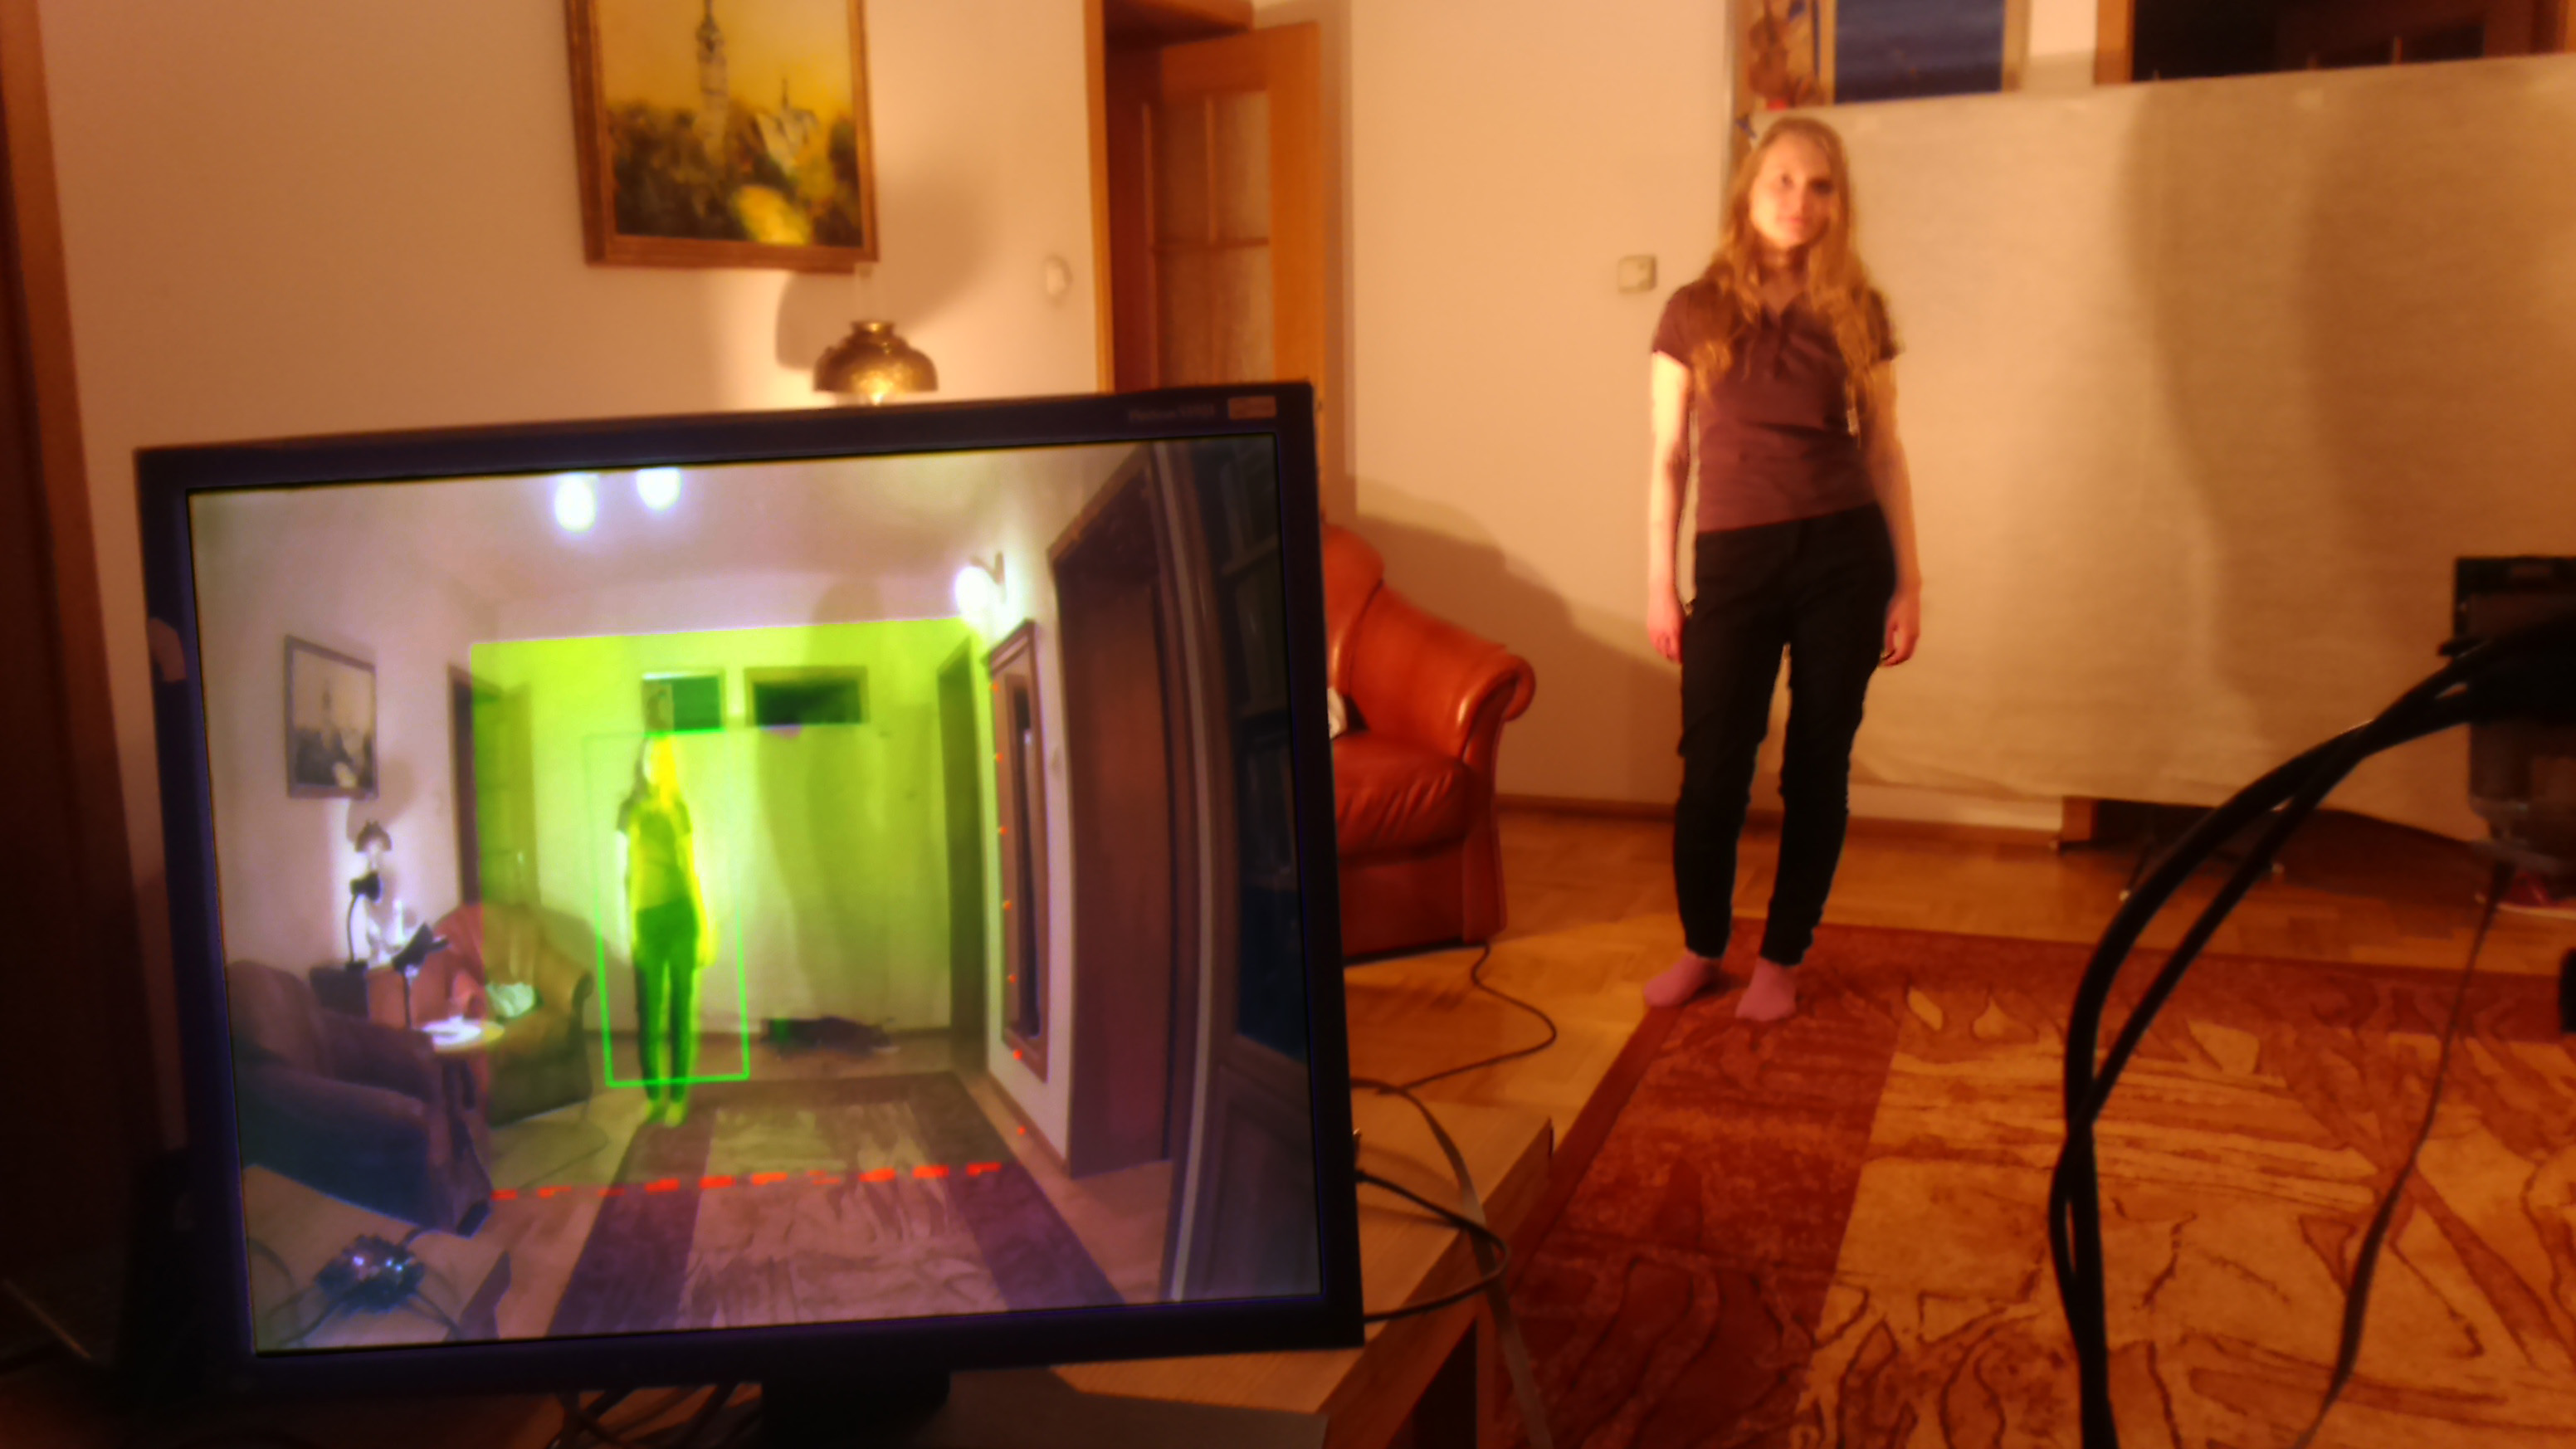
\includegraphics[width=0.8\linewidth]{images/workingSystem.jpg}
\caption[Działający system.]{Działający system.}
\label{fig:workingSystem}
\end{figure}

%TODO  no ale jakby to dla 30/60 fps... to już tak pięknie nie jest %% TT Mam w zapasie moduł który liczy gradienty oraz przedział i histogram pojedynczego piksela, tylko dodanie go powoduje że układ jest niesyntezowalny 
W tabeli \ref{tab:fpgautilization} zostało przedstawione wykorzystanie zasobów logiki programowalnej. 
\begin{table}[]
\centering
\caption{Wykorzystane zasoby logiki programowalnej.}
\label{tab:fpgautilization}
\begin{tabular}{|l|l|l|l|}
\hline
Element & Wykorzystane & Dostępne & \% \\ \hline %TODO OK po polsku
LUT & 12583 & 17600 & 71,49 \\ \hline 
LUTRAM & 617 & 6000 & 10,28 \\ \hline 
FF & 19924 & 35200 & 56,60 \\ \hline
BRAM & 25,50 & 60 & 42,50 \\ \hline
DSP & 36 & 80 & 45,00 \\ \hline
IO & 43 & 100 & 43,00 \\ \hline
BUFG & 7 & 32 & 21,88 \\ \hline
MMCM & 1 & 2 & 50,00 \\ \hline
PLL & 1 & 2 & 50,00 \\ \hline
\end{tabular}
\end{table}

%TODO Podsumowanie oraz wskazanie dalszych kierunków pracy
%TODO Dodatek A - spis zawartości CD
%TODO Dodatek B - opis informatyczny projektu
